\documentclass[tikz,border=6pt]{standalone}
\usepackage{tikz}

\begin{document}
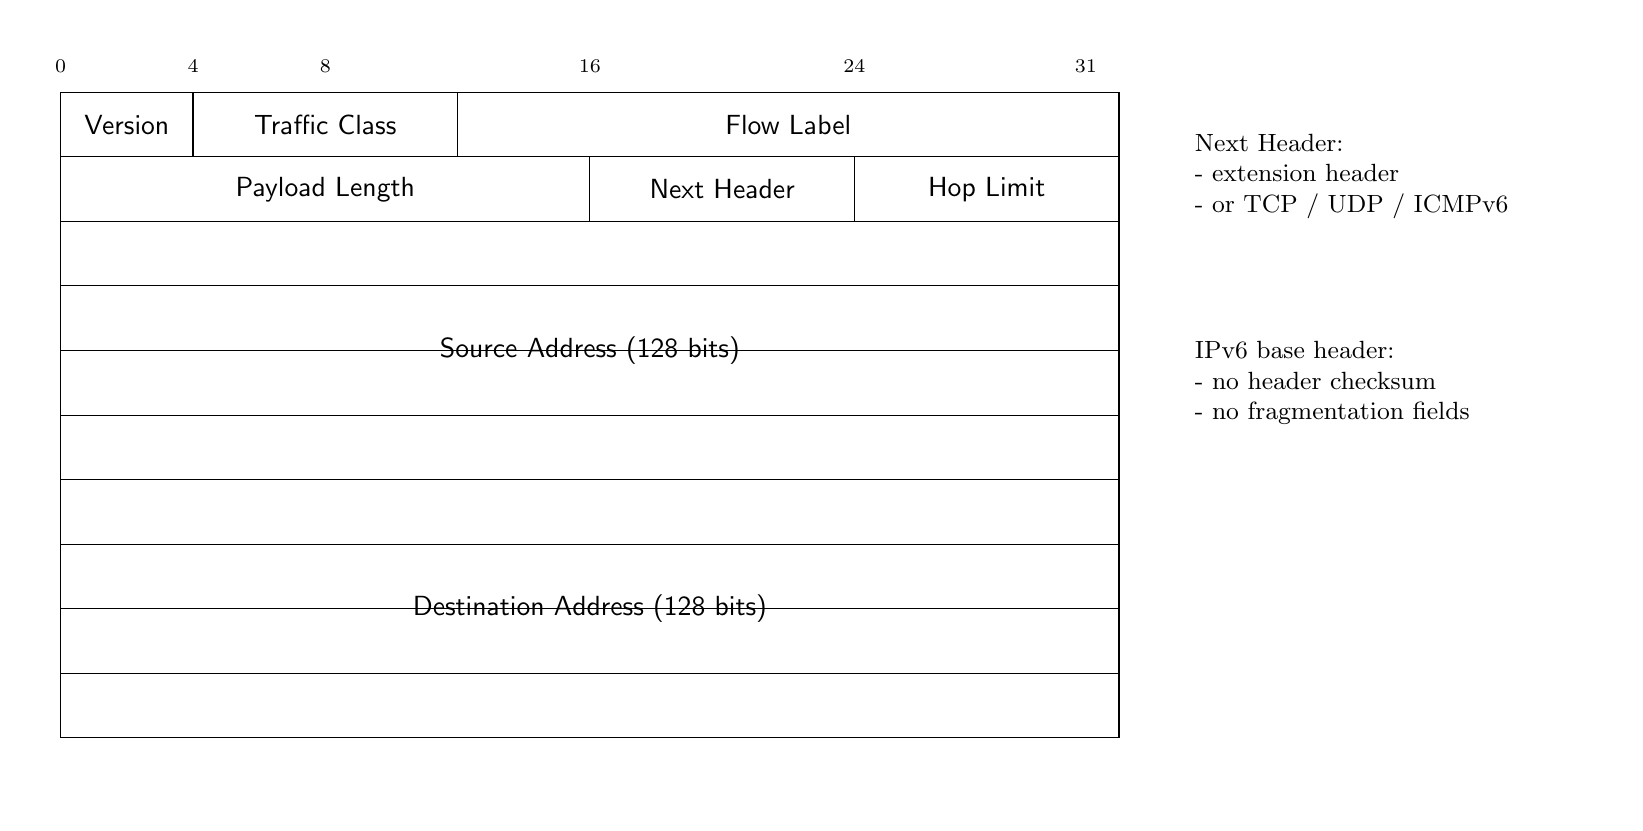
\begin{tikzpicture}[
  x=0.42cm,
  y=0.82cm,
  font=\sffamily,
  bitlabel/.style={font=\scriptsize}
]

% White background
\fill[white] (-1,-1) rectangle (47,11);

% Bit labels
\foreach \x/\lbl in {0/0,4/4,8/8,16/16,24/24,31/31} {
  \node[bitlabel, anchor=south] at (\x,10.15) {\lbl};
}

% 10 rows total
\foreach \y in {0,1,2,3,4,5,6,7,8,9} {
  \draw (0,\y) rectangle (32,\y+1);
}

% Top row splits
\draw (4,9) -- (4,10);
\draw (12,9) -- (12,10);

% Second row splits
\draw (16,8) -- (16,9);
\draw (24,8) -- (24,9);

% Labels
\node at (2,9.5) {Version};
\node at (8,9.5) {Traffic Class};
\node at (22,9.5) {Flow Label};

\node at (8,8.5) {Payload Length};
\node at (20,8.5) {Next Header};
\node at (28,8.5) {Hop Limit};

\node at (16,6) {Source Address (128 bits)};
\node at (16,2) {Destination Address (128 bits)};

% Side notes
\node[align=left, anchor=west, font=\small] at (34,8.7) {%
Next Header:\\
- extension header\\
- or TCP / UDP / ICMPv6
};

\node[align=left, anchor=west, font=\small] at (34,5.5) {%
IPv6 base header:\\
- no header checksum\\
- no fragmentation fields
};

\end{tikzpicture}
\end{document}